% Since this a solution template for a generic talk, very little can
% be said about how it should be structured. However, the talk length
% of between 15min and 45min and the theme suggest that you stick to
% the following rules:  

% - Exactly two or three sections (other than the summary).
% - At *most* three subsections per section.
% - Talk about 30s to 2min per frame. So there should be between about
%   15 and 30 frames, all told.


\section{Applications}

\subsection{Information density and redundancy}

\begin{frame}
  \begin{definition}
    \begin{itemize}
      \item Natural language \(L\).
      \item Stochastic variable \(\stoch P^n_L\) of strings of length \(n\).
      \item (Alphabet \(P_L\).)
      \item Entropy of \(L\) defined as
        \begin{align*}
          H_L = \lim_{n\to \infty}\frac{H(\stoch P^n_L)}{n}.
        \end{align*}
      \item Redundancy in \(L\) is
        \begin{align*}
          R_L = 1 - \frac{H_L}{\log |P_L|}.
        \end{align*}
    \end{itemize}
  \end{definition}
\end{frame}

\begin{frame}
  \begin{remark}
    Meaning we have \(H_L\) bits per character in \(L\).
  \end{remark}

  \begin{example}[\cite{Shannon1948amt}]
    \begin{itemize}
      \item Entropy of 1--1.5 bits per character in English.
      \item Redundancy of approximately \(1 - \frac{1.25}{\log 26} \approx 
          0.73\).
    \end{itemize}
  \end{example}

\end{frame}

\begin{frame}
  \begin{example}[\cite{Shannon1948amt}]
    Two-dimensional cross-word puzzles requires redundancy of approximately 
    \(0.5\).
  \end{example}

  \begin{example}
    \begin{itemize}
      \item Redundancy of \enquote{SMS languages} is lower than for 
        \enquote{non-SMS languages}.

      \item Compare \enquote{också} and \enquote{oxå}.

    \end{itemize}
  \end{example}

  \begin{remark}
    \begin{itemize}
      \item Lower redundancy is more space-efficient.
      \item Incurs more errors.
    \end{itemize}
  \end{remark}
\end{frame}

%\begin{frame}
%  \begin{itemize}
%    \item Detta säger också att vi kan uppskatta entropin för en given 
%      Markovprocess.
%
%    \item Shannon modellerade språket som en Markovprocess i sin artikel 
%      \cite{Shannon1948amt}.
%
%    \item Vi kan även beräkna entropin för ett givet tillstånd i en 
%      Markovprocess genom betingad entropi.
%
%  \end{itemize}
%\end{frame}

\subsection{Passwords}

\begin{frame}
  \begin{block}{Idea~\cite{Komanduri2011opa}}
    \begin{itemize}
      \item Look at different aspects of passwords individually, then 
        summarize.
      \item Can use \(H(x_1, x_2, \ldots, x_n) \leq H(x_1) + H(x_2) + \cdots 
          + H(x_n)\).
      \item This allows us to reason about bounds.
    \end{itemize}
  \end{block}
\end{frame}

\begin{frame}
  \begin{example}
    \begin{itemize}
      \item We can look at properties such as:
        \begin{itemize}
          \item length,
          \item number of and placement of character classes,
          \item the actual characters,
          \item \dots
        \end{itemize}
    \end{itemize}
  \end{example}

  \pause{}

  \begin{remark}
    \begin{itemize}
      \item These are \emph{not independent}.
      \item The sum will be an \emph{upper bound}.
    \end{itemize}
  \end{remark}
\end{frame}

\begin{frame}
  \begin{remark}
    \begin{itemize}
      \item With an upper bound we know it's not possible to do better.
      \item With an average we know how well most users will do.
      \item With a lower bound we have a guarantee --- not possible!
    \end{itemize}
  \end{remark}
\end{frame}

\begin{frame}
  \begin{remark}
    \begin{itemize}
      \item If a password policy yields low entropy, it implies it's bad.
      \item If a password policy yields high entropy, it \emph{doesn't} imply 
        that it's good.
    \end{itemize}
  \end{remark}

  \pause

  \begin{exercise}
    Why?
  \end{exercise}
\end{frame}

\begin{frame}
  \begin{figure}
    \includegraphics[height=0.7\textheight]{password_strength.png}
    \caption{xkcd's strip on password strength.
    Picture: xkcd~\cite{xkcd936}.}
  \end{figure}
\end{frame}

%\begin{frame}{En förklaring av xkcd}
%  \begin{itemize}
%    \item Vi har 1 miljon engelska ord: ger \(\log 10^6 \approx 20\) bitar 
%      entropi.
%      (xkcd använder 16 bitar, vilket ger ca 70\,000 ord, alla ord i engelskan 
%      är inte vanliga.)
%
%    \item Vi kan ha inledande versal: ger 1 bit entropi.
%
%    \item Vi har några vanliga substitutioner: uppskattningsvis 10 stycken, 
%      d.v.s.~3 bitar entropi.
%
%    \item Vi har specialtecken (ej substitution): uppskattningsvis 4 bitar 
%      entropi.
%
%    \item Vi har siffror: \(\log 10\approx 3\).
%
%    \item Ordningen på specialtecknet och siffran: ger 1 bit entropi.
%
%    \item Totalt 32 bitar entropi:
%      \begin{itemize}
%        \item Tar minst 50 dagar med 1\,000 gissningar per sekund.
%        \item Tar strax över en timme med 1\,000\,000 gissningar per sekund.
%      \end{itemize}
%
%  \end{itemize}
%\end{frame}

\begin{frame}
  \begin{example}[Standard password]
    \begin{itemize}
      \item We have
        \begin{itemize}
          \item 26 alphabetic characters,
          \item 10 numbers,
          \item 10 special characters (approximately).
        \end{itemize}

      \item This yields \(\log( 2\times 26 + 10 + 10 ) = \log 72 \approx 
          \SI{6}{\bit}\) per password character.

      \item A 10-character \emph{uniformly randomly} generated password 
        contains \SI{60}{\bit}.
    \end{itemize}
  \end{example}

  \pause{}

  \begin{remark}
    What happens when we require two upper and two lower-case characters, two 
    numbers must be included?
  \end{remark}
\end{frame}

\begin{frame}
  \begin{example}[Four-word passphrase]
    \begin{itemize}
      \item We have 125\,000 words in the standard Swedish dictionary.
      \item This yields \(\log 125\,000\approx \SI{17}{\bit}\) per word.
      \item A four-word \emph{uniformly randomly} generated passphrase contains
        \SI{68}{\bit}.
    \end{itemize}
  \end{example}
\end{frame}

\begin{frame}
  \begin{example}[Random sentence]
    \begin{itemize}
      \item We estimated the entropy per character in a language.
      \item It was approximately \(\SI{1.25}{\bit}\) for English.
      \item A 20-character \emph{uniformly randomly} generated sentence would 
        yield \SI{25}{\bit}.
    \end{itemize}
  \end{example}
\end{frame}

\begin{frame}
  \begin{remark}
    \begin{itemize}
      \item All these require uniform randomness.
      \item Humans are bad at remembering random things.
      \item Thus they will choose non-randomly.
      \item The entropy will thus be (possibly much) lower.
    \end{itemize}
  \end{remark}
\end{frame}

\subsection{Research about human chosen passwords}

\begin{frame}
  \begin{example}[\citetitle{Bonneau2012lpo}~\cite{Bonneau2012lpo}]
    \begin{itemize}
      \item Investigates how linguistics affect the choice of multi-word 
        passphrases.

      \item Users don't choose them randomly, prefer adapted to natural 
        language.

      \item \enquote{correct horse battery staple} is preferred to 
        \enquote{horse correct battery staple} since the first is more 
        grammatically correct.
    \end{itemize}
  \end{example}
\end{frame}

\begin{frame}
  \begin{example}[\citetitle{Kuo2006hso}~\cite{Kuo2006hso}]
    \begin{itemize}
      \item Studied how users creates easy-to-remember passwords.

      \item Also investigated the strength of phrase-based passwords.

      \item E.g.\ Google's example \enquote{To be or not to be, that is the 
          question}\footnote{%
          URL\@: 
          \protect\url{http://www.lightbluetouchpaper.org/2011/11/08/want-to-create-a-really-strong-password-dont-ask-google/}.
        } which results in \enquote{2bon2btitq}.

      \item This particular password has apparently been used by many \dots
    \end{itemize}
  \end{example}
\end{frame}

\begin{frame}
  \begin{remark}
    \begin{itemize}
      \item There is a PhD thesis on the topic of guessing passwords: 
        \fullcite{GuessingHumanChosenSecrets}.
      \item There is even a conference dedicated to passwords: PasswordsCon.
    \end{itemize}
  \end{remark}
\end{frame}

\subsection{Identifying information}

\begin{frame}
  \begin{example}
    Do we get more information from zodiac signs or birthdays?
    \begin{align*}
      -\sum_{\mathclap{\text{zodiacs}}} \frac{1}{12} \log\frac{1}{12} &= \log 12 
      \approx 3.58 \\
      &< -\sum_{\mathclap{\text{days of year}}} \frac{1}{365} \log\frac{1}{365} 
      = \log 365 \approx 8.51.
    \end{align*}
  \end{example}
\end{frame}

\begin{frame}
  \begin{exercise}
    How much information do we need to uniquely identify an individual?
  \end{exercise}
\end{frame}

\begin{frame}
  \begin{example}
    \begin{itemize}
      \item Sometime during 2011 there were \(n = 6\,973\,738\,433\)\footnote{%
          According to the World Bank.
        } people on earth.

      \item To give everyone a unique identifier we need \(\log n\approx 
          32.7\approx 33\) bits of information.
    \end{itemize}
  \end{example}
\end{frame}

\begin{frame}
  \begin{block}{Identifying information in browsers}
    \begin{itemize}
      \item Electronic Frontier Foundation (EFF) studied~\cite{Eckersley2010hui} 
        how much information a web-browser shares.

      \item You can try your browser in \url{http://panopticlick.eff.org/}.
    \end{itemize}
  \end{block}

  \pause{}

  \begin{example}[My browser]
    \begin{itemize}
      \item My Firefox-browser with all addons gave 21.45 bits of entropy.

      \item Then the number of tested users were 2\,860\,696.
    \end{itemize}
  \end{example}
\end{frame}

\begin{frame}
  \begin{figure}
    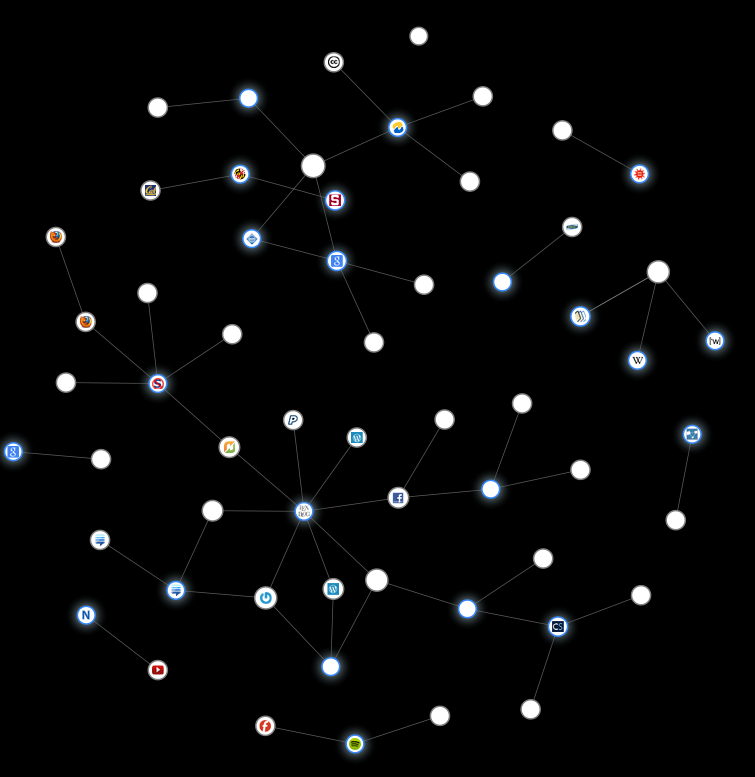
\includegraphics[height=0.7\textheight]{collusion.png}
    \caption{Screenshot from Collusion (now Lightbeam) for Firefox.
      Map over all pages that track me using this information.}
  \end{figure}
\end{frame}


%%%%%%%%%%%%%%%%%%%%%%

\subsection*{References}
\begin{frame}[allowframebreaks]
	\small
  \printbibliography{}
\end{frame}

